\documentclass[12pt]{article}
\usepackage{amsmath, amssymb, graphicx, hyperref}
\usepackage{indentfirst}
\usepackage[sorting=none]{biblatex}
\bibliography{refs}
\title{Plasma Mirrors}
\author{Harikesh}
\date{\today}

\newenvironment{changemargin}[2]{%
\begin{list}{}{%
\setlength{\topsep}{0pt}%
\setlength{\leftmargin}{#1}%
\setlength{\rightmargin}{#2}%
\setlength{\listparindent}{\parindent}%
\setlength{\itemindent}{\parindent}%
\setlength{\parsep}{\parskip}%
}%
\item[]}{\end{list}}
\begin{document}
\begin{titlepage}
    \begin{changemargin}{-2cm}{-2cm}
        \begin{figure}
            
\includegraphics[width=5cm, height=5cm]{logo.png}
            \centering
        \end{figure}
        \begin{center}
            \textbf{\Large{Department of Physics, IIT Delhi}}\\
            \vspace*{1cm}
            \textbf{\Large{Course Code : PYD561}}\\
            \vspace*{0.2cm}
            \textbf{\Large {Semester - III, 2022-23}}\\
            \vspace*{1cm}
            \textbf{\LARGE{Plasma Mirrors}}\\
            \vspace*{1cm}
            \textbf{\Large{Kulwinder Kaur (2021PHS7190)}}\\
            \vspace*{0.2cm}
            \textbf{\Large {Harikesh Kushwaha (2021PHS7181)}}\\
            \vspace*{1cm}
            \textbf{\Large {Adviser: Prof. Vikrant Saxena}}\\
            \vspace*{2cm}
        \end{center}
        \begin{flushleft}


            \textbf{Signature of student 1: \ldots \ldots \ldots}\\
            \vspace*{1cm}
            \textbf{Signature of student 2: \ldots \ldots \ldots}
            \hspace*{3cm}
            \textbf{Signature of the adviser: \ldots \ldots \ldots}
        \end{flushleft}
    \end{changemargin}
\end{titlepage}
\newpage
\begin{changemargin}{-2cm}{-2cm}
    \section{Introduction And Motivation}
    There is great interest in high intensity physics where the study of interaction of light with matter at Ultra High Light Intensity (UHLI) is performed. The main goal is to achieve high intensity which give access to novel physical regimes.\cite{henri}
    Intensity of laser in order of $10^{23} \; W/cm^{-2}$ has been reached experimentally with the CoReLS petawatt (PW) laser.\cite{highintensity}. The next step is to push forward these intensities above $10^{25}W/cm^{-2}$. Above this limit, quantum electrodynamics effects start playing a major role on the dynamics of electrons. Intensity level of $10^{29}W/cm^{-2}$ corresponds to the Schwinger field. At this field, light starts generating electron positron pair out of vacuum. Vacuum starts acting like a nonlinear medium and its refractive index becomes a function of light intensity. These physical regimes are barely, if at all, explored in lab.

    One way to get these UHLI is by using plasma mirrors (PM). When a laser pulse is incident upon plasma, it reflects if the density of plasma is high, forming PM. Upon reflection from plasma the laser field, because of pondermotive force, propels a relativistic oscillation of the PM which results in periodic temporal compression of the reflected field (Doppler effect). These oscillations results in generation of high harmonics of the incident laser frequency.\cite{lichters} Experiments have been performed showing generation of high harmonics of order up to 141st of Nd glass laser\cite{hormonics1}, 109th of Ti sapphire laser\cite{hormonics2}, and 37th of krypton fluoride laser\cite{hormonics3}.

    Here, the generation of harmonics of incident laser pulse by interaction of a high intensity laser pulse with a step boundary overdense plasma layer is studied and the effect of variuos parameters on the generated high hormonics is investigated. For this, fully relativistic particle in cell simulations are performed using \textit{EPOCH}. Already, variuos experiments and simulations have been performed to study how high hormonics are changed by using different polarization of laser pulse \cite{polarization1} \cite{polarization2}, different PM shapes \cite{henri}, two color laser pulses \cite{two-color1} \cite{two-color2}. In this article, we study the effect of plasma density, laser intensity, envelope and pulse duration on generated high harmonics.
    \section{Methodology}

    The simulation uses \textit{EPOCH}, a parallised, second order and fully relativistic implementation of particle in cell algorithm.\cite{EPOCH} Though \textit{EPOCH} is implemented in 3D, the current simulation is performed in 1D3V only.
    \subsection{Simulation Parameters}
    We want to study the effect of various plasma and laser parameters on the generated high harmonics. The parameters which are constant throughout the entire experimentation are these:
    The simulation box extends for $40 \lambda _l$ (from $-20 \lambda _l$ to $20 \lambda _l$), where $\lambda_l$ is the laser wavelength taken as $1\mu m$ and has total 16000 cells, i.e., 400 cells per wavelength. The plasma is placed at $x=0$ and with a thickess of $\lambda_l$. Number of particles per cell are 100.
    For most of the simulations the pulse duration is $T = 20 \tau$ and simulation is run till $T_{end} = 40 \tau$. Here $\tau$ is the time period of laser pulse.\\
    Some parameters in the simulations are varied to observe their effect on high harmonic generation. These are listed below:\\
    \textbf{Laser Envelope}:
    Three laser envelopes are used. They are:\\
    \noindent
    1. Sine Sqaured
    \begin{equation}\label{sin-sq-env}
        P(t)=
        \begin{cases}
             & \sin^2(\pi t/T) \text{ for } 0 \leq t \le T \\
             & 0         \;      \text{ otherwise }
        \end{cases}
    \end{equation}
    2. Gaussian
    \begin{equation}\label{gaussian-env}
        P(t)=
        \begin{cases}
             & e^{\frac{-(t-T/2)^2}{2(0.2T)^2}} \text{ for } 0 \leq t \le T \\
             & 0         \;      \text{ otherwise }
        \end{cases}
    \end{equation}
    3. Triangular
    \begin{equation}\label{triangle-env}
        P(t)= 2\times
        \begin{cases}
             & t/T \text{ for } 0 \leq t \le T/2    \\
             & 1-t/T \text{ for } T/2 \leq t \le T  \\
             & 0         \;      \text{ otherwise }
        \end{cases}
    \end{equation}
    \noindent
    \textbf{Plasma Density}:
    The ratio of plasma density to the critical density is varied as $7$ and $4$.\\
    \noindent
    \textbf{Normalized Vector Potential}:
    Normalized Vector Potential, $a_0$, is varied as 0.5 and 1.\\
    \noindent
    \textbf{Pulse Duration}:
    The pulse duration is varied as $5\tau$, $10\tau$, $20\tau$, $30\tau$.

    \section{Result and Discussion}
    A number of simulations are performed to study the effect of various parameters discussed above on the generated high harmonics. The results are presented in the following subsections.
    % The following figure shows the generation of harmonic when short laser pulse is reflected from plasma with density eqaul to four times the critical density. The laser envelope is sine squared and the normalized vector potential is 0.5.

    % \label{fig:base}
    % 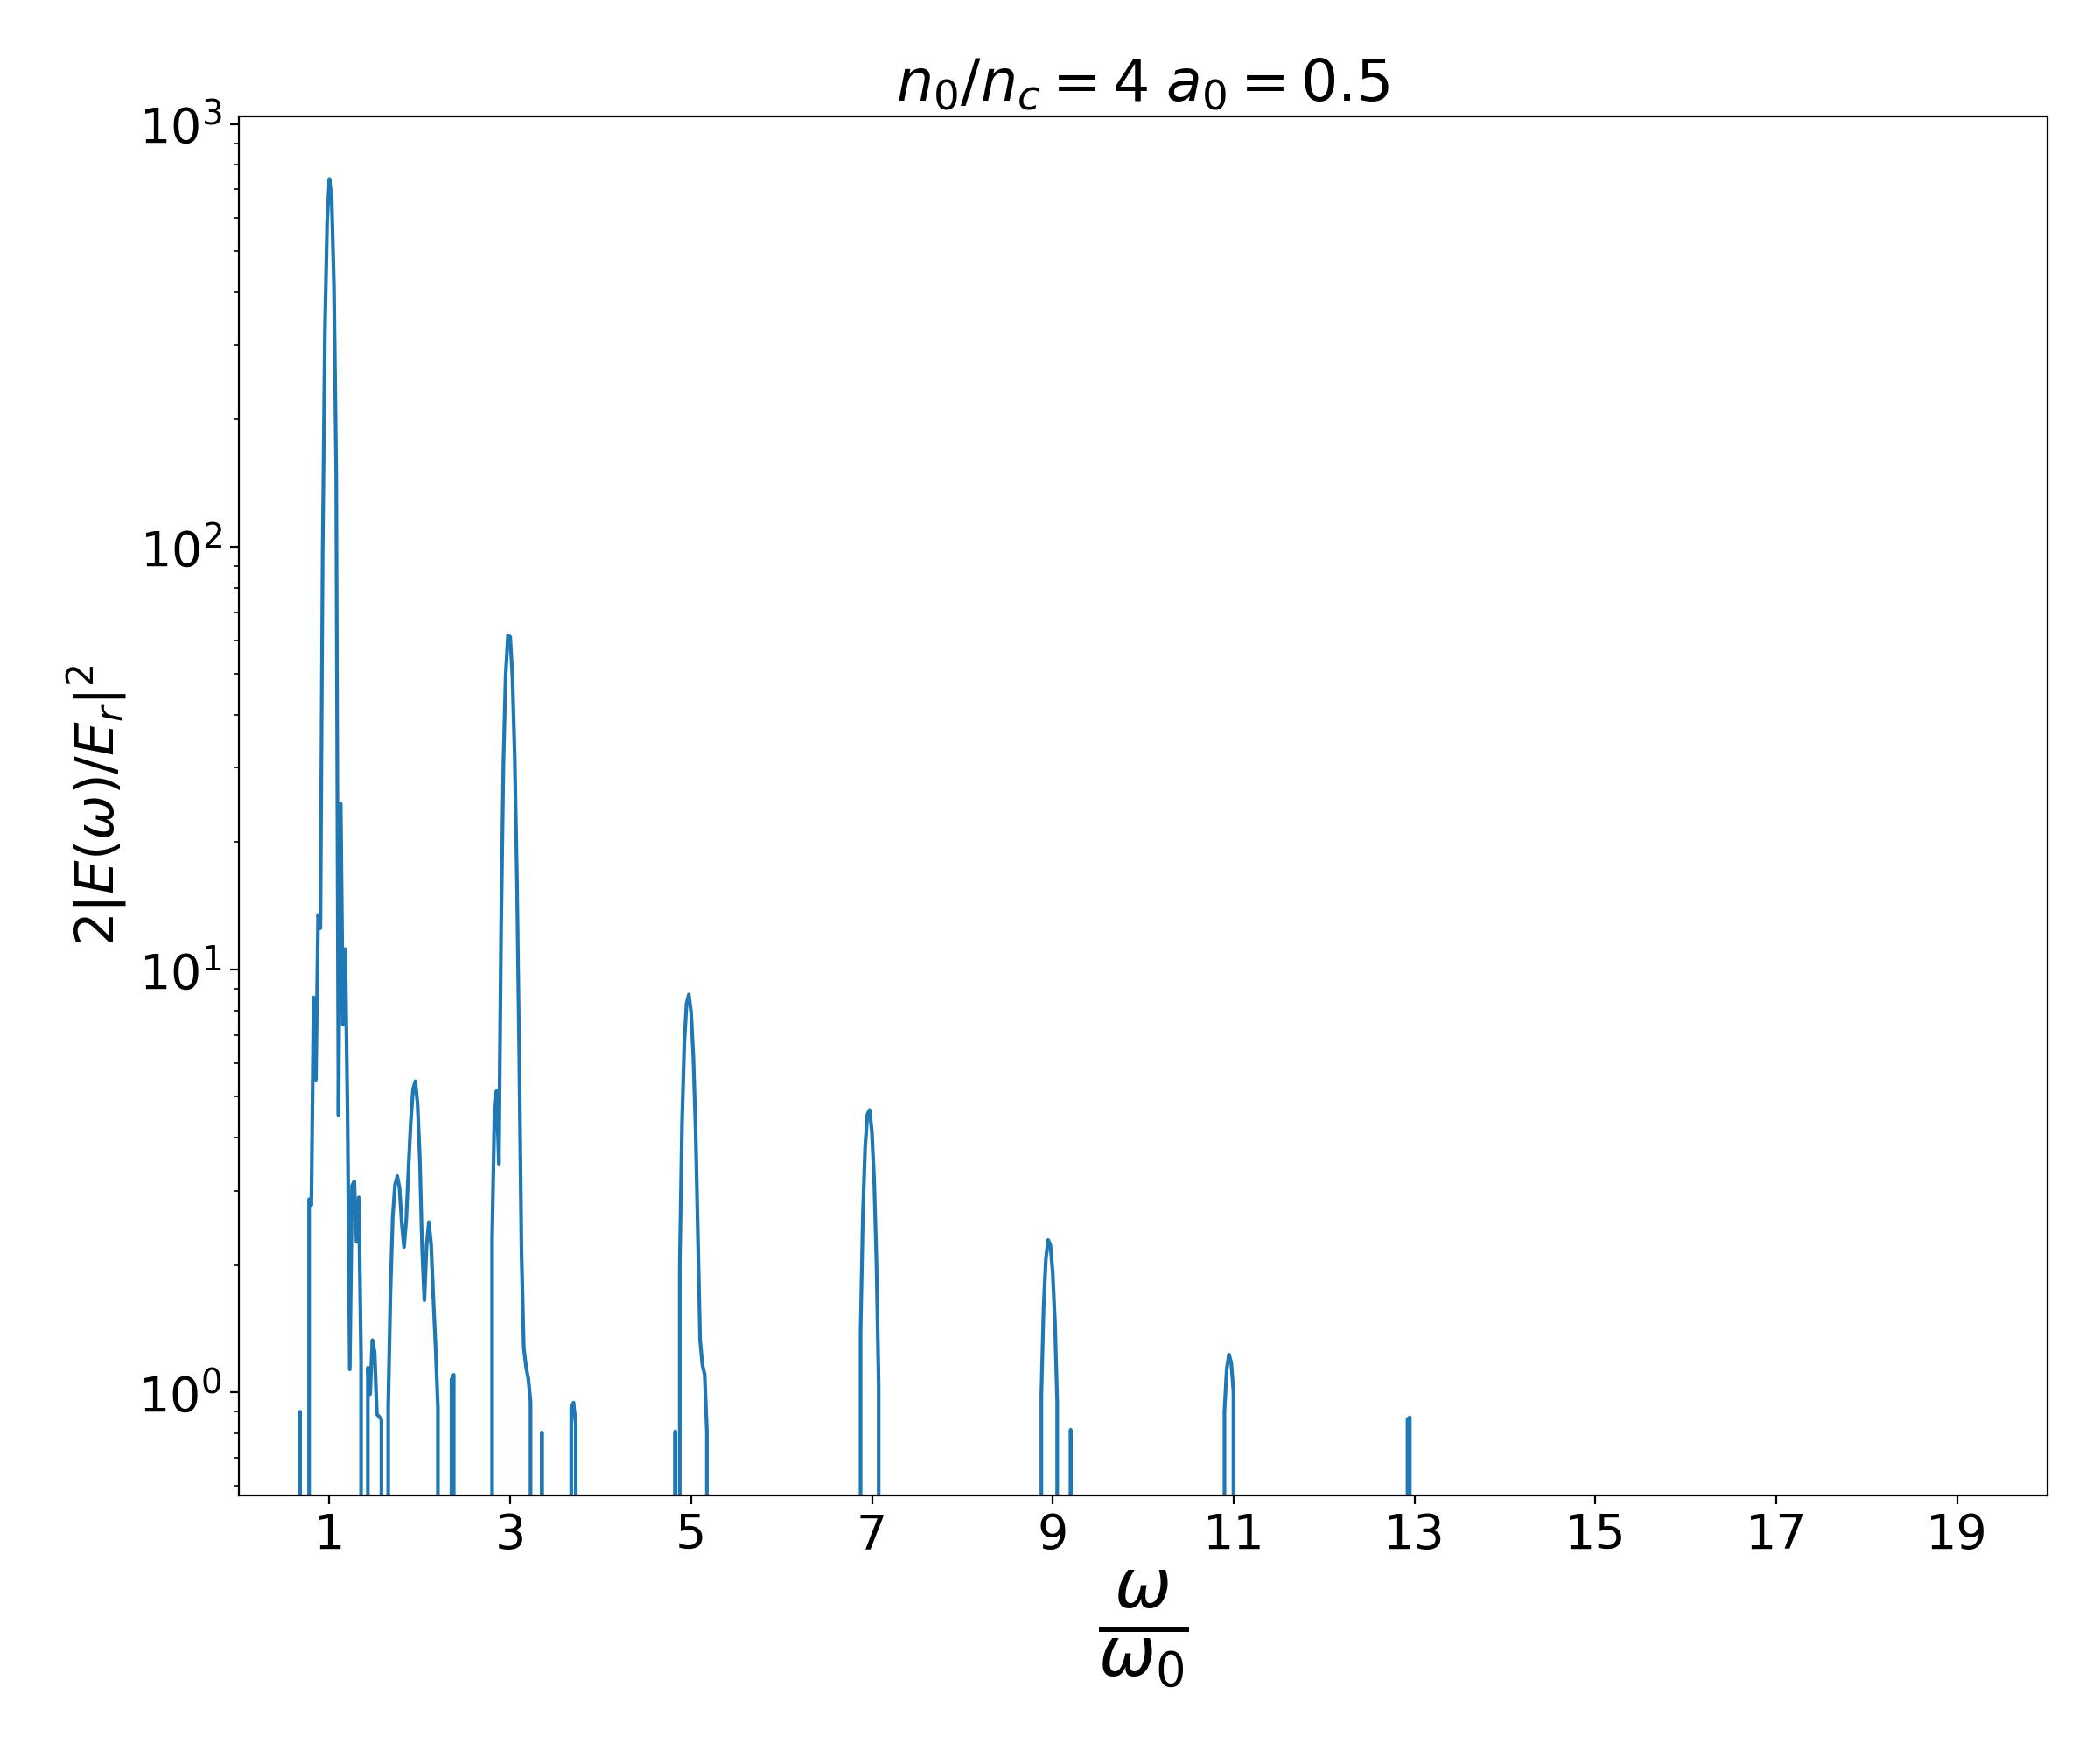
\includegraphics[width=0.8\textwidth]{images/base.jpg}

    % A number of simulations is performed to study the effect of different parameters on the high harmonic generation. The above case is used as a base to discuss the changes due to the  variation of different parameters.
    \subsection{Effect of Plasma Density}
    Increasing plasma density decreases the number of harmonics generated. The amplitude of the harmonics also decreases. The Figure \ref{fig:density} shows the effect of plasma density on the harmonics generated.
    \begin{figure}[h]
        \centering
        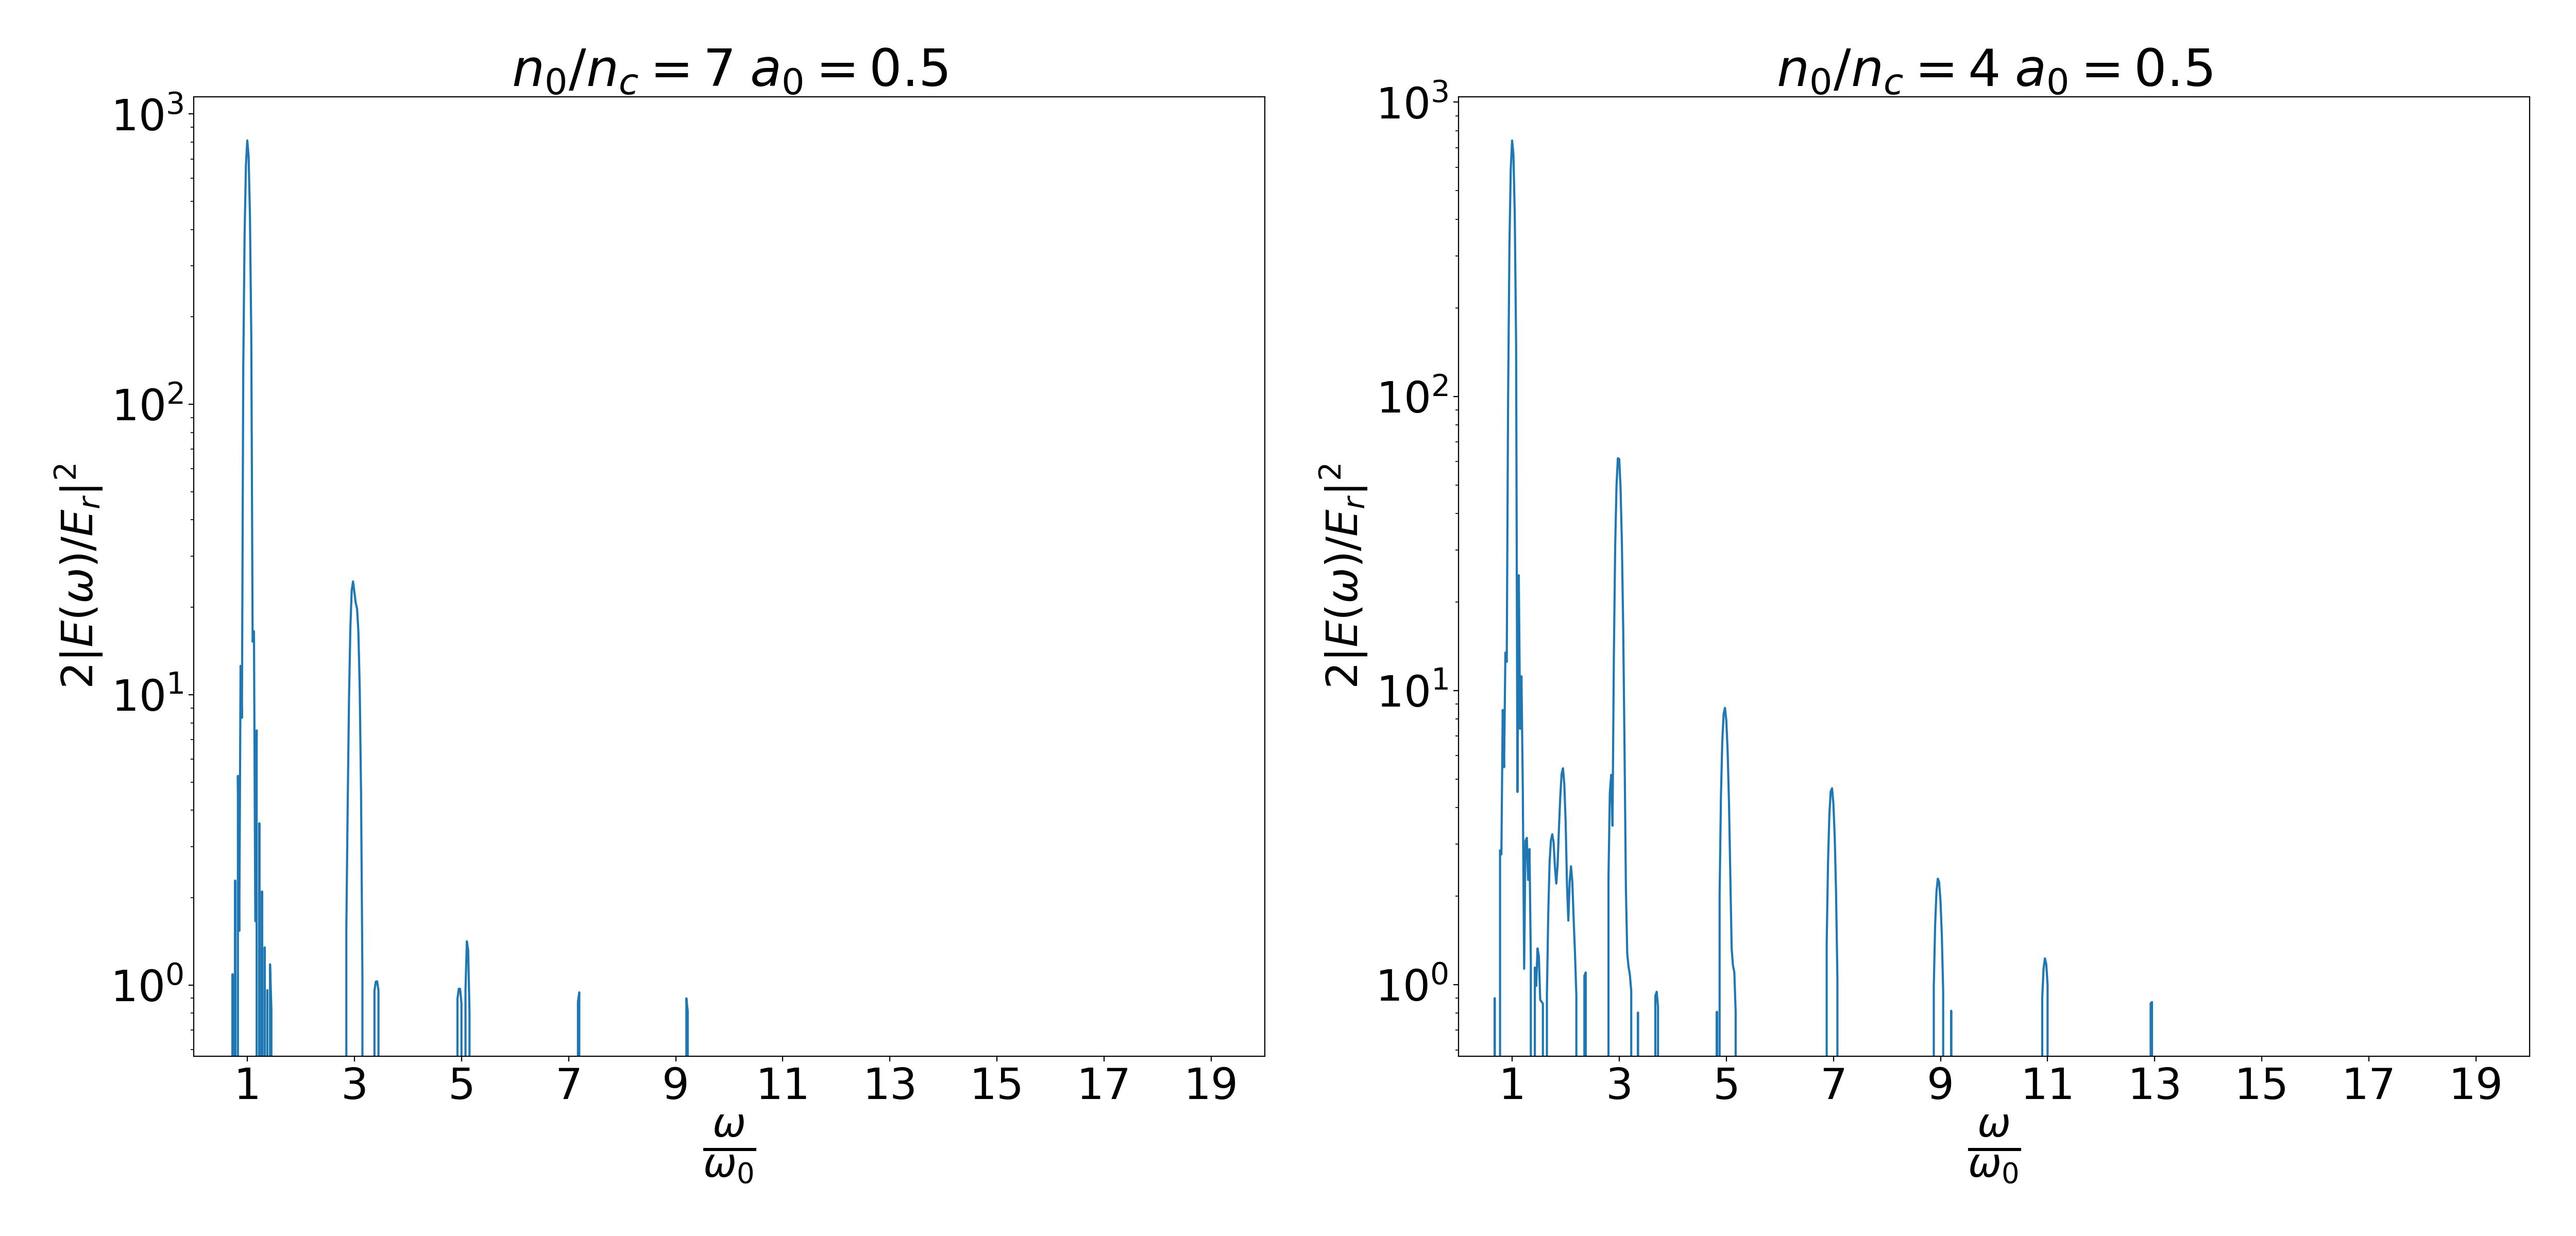
\includegraphics[width=1.0\textwidth]{images/density.jpg}
        \caption{Effect of laser density on the harmonics generated.}
        \label{fig:density}
    \end{figure}
    \subsection{Effect of Laser Intensity}
    Increasing the laser intensity increases the number of harmonics generated. The amplitude of the harmonics also increases. The Figure \ref{fig:intensity} shows the effect of laser intensity on the harmonics generated.

    \begin{figure}[h]
        \centering
        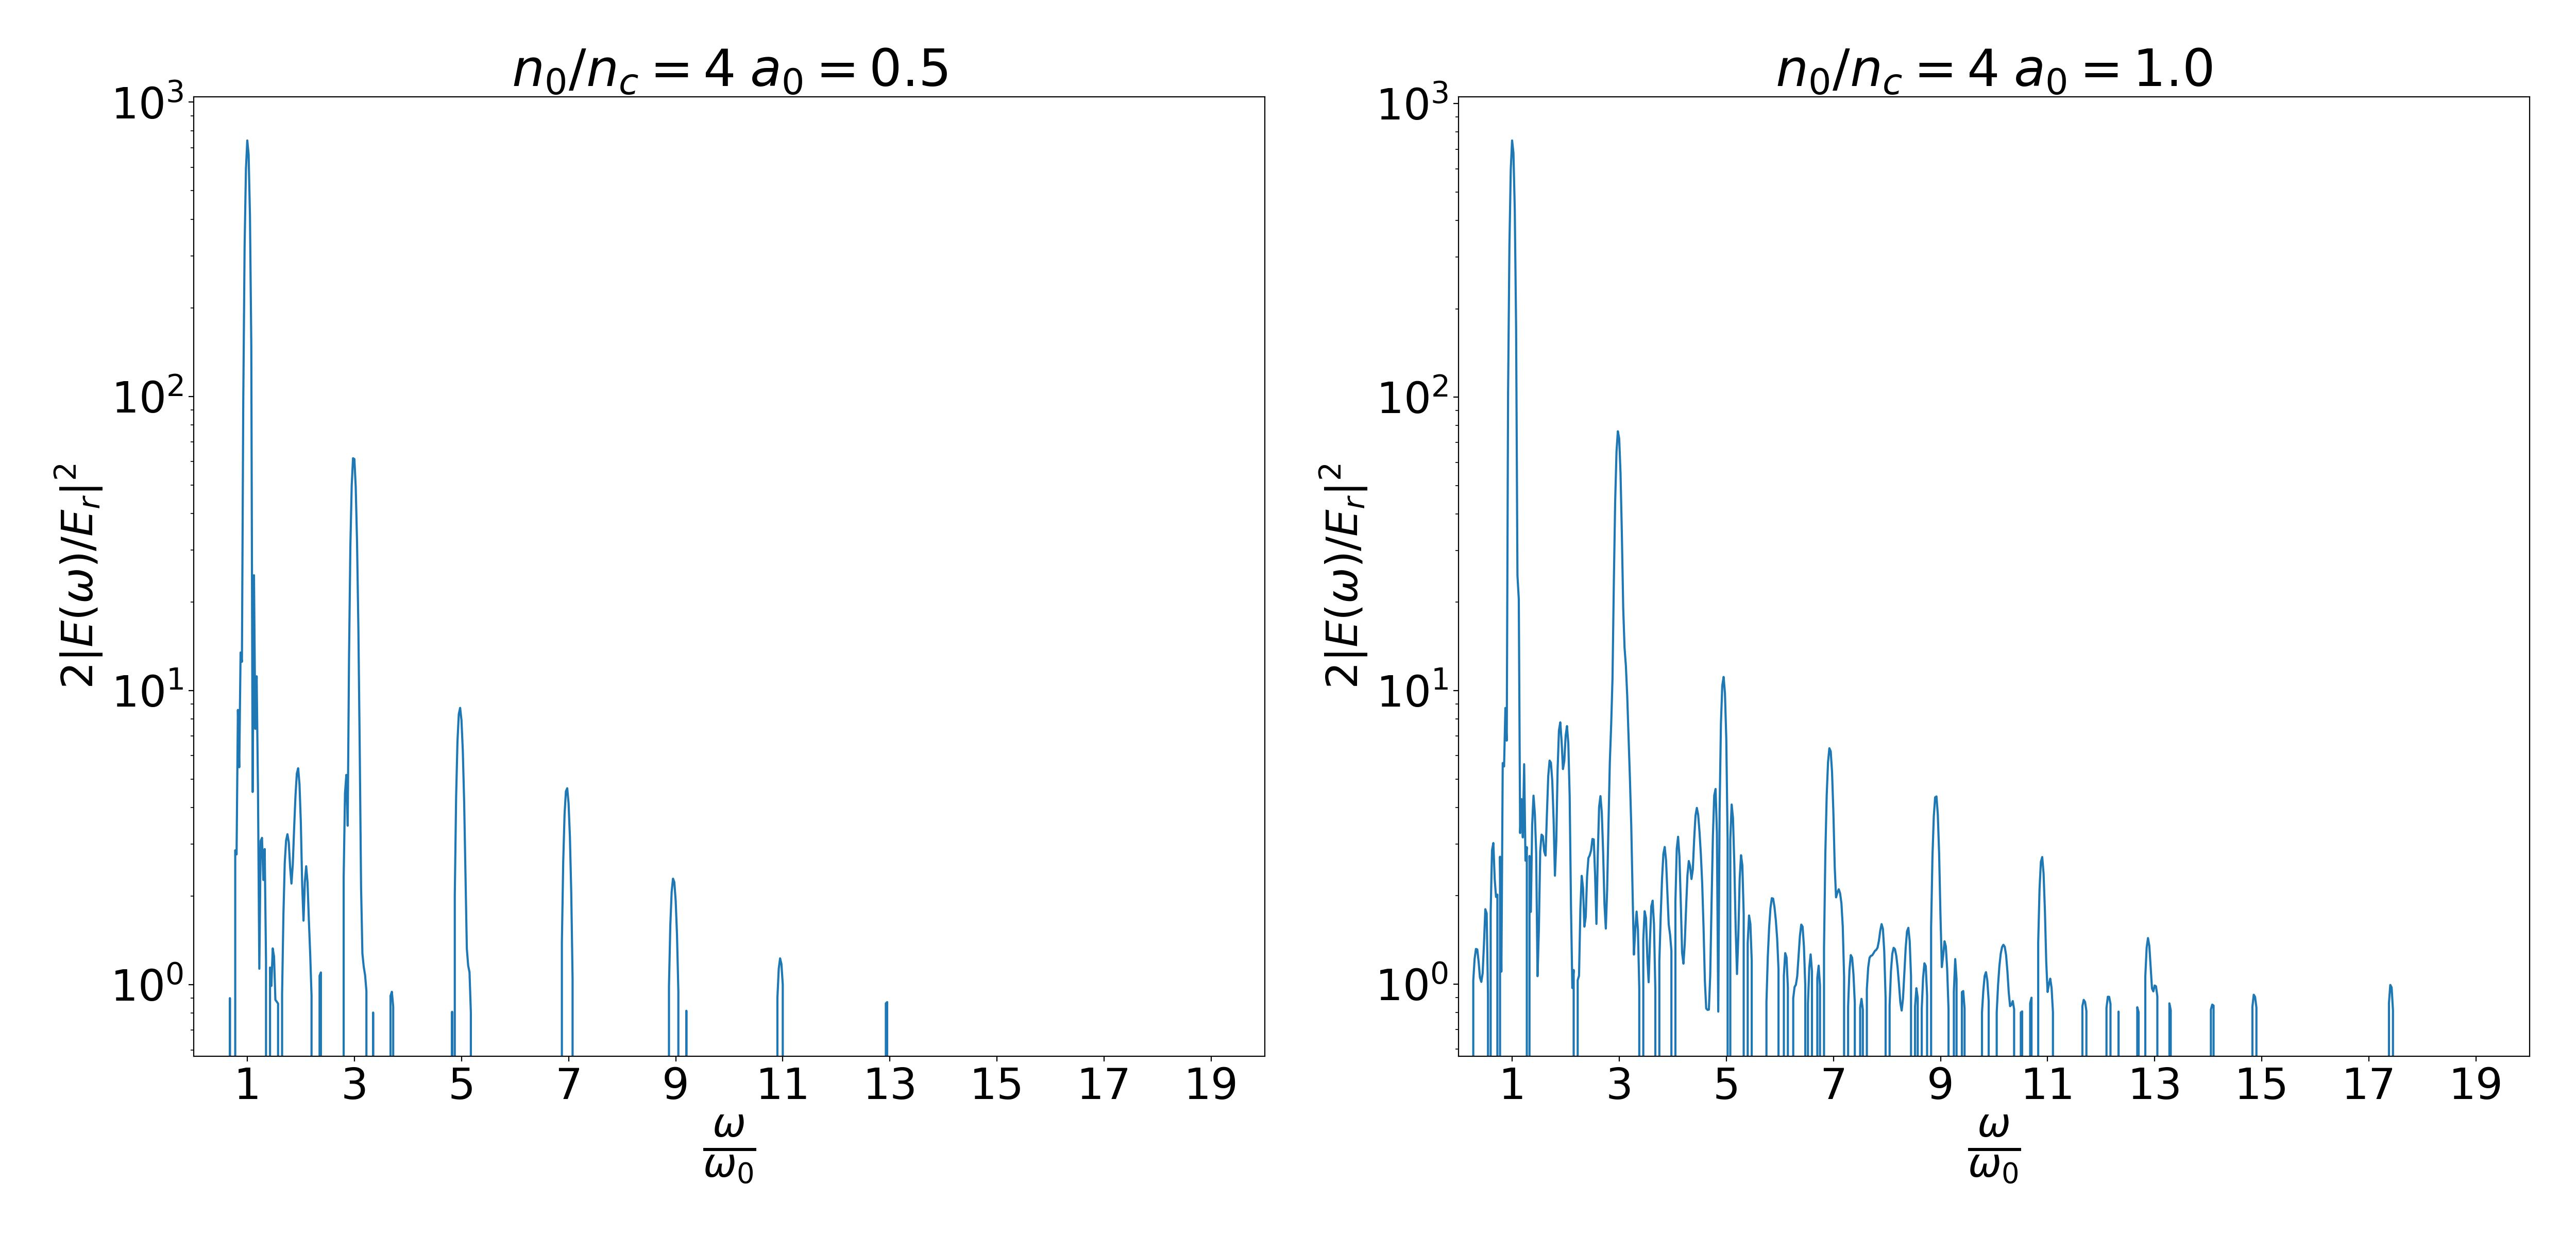
\includegraphics[width=1.0\textwidth, height=0.4\textwidth]{images/intensity.jpg}
        \caption{Effect of plasma intensity on the harmonics generated.}
        \label{fig:intensity}
    \end{figure}
    \subsection{Effect of Laser Envelope}
    The laser envelope does not seem to have any effect at all. See the Figure \ref{fig:env}.
    \begin{figure}[t]
        \centering
        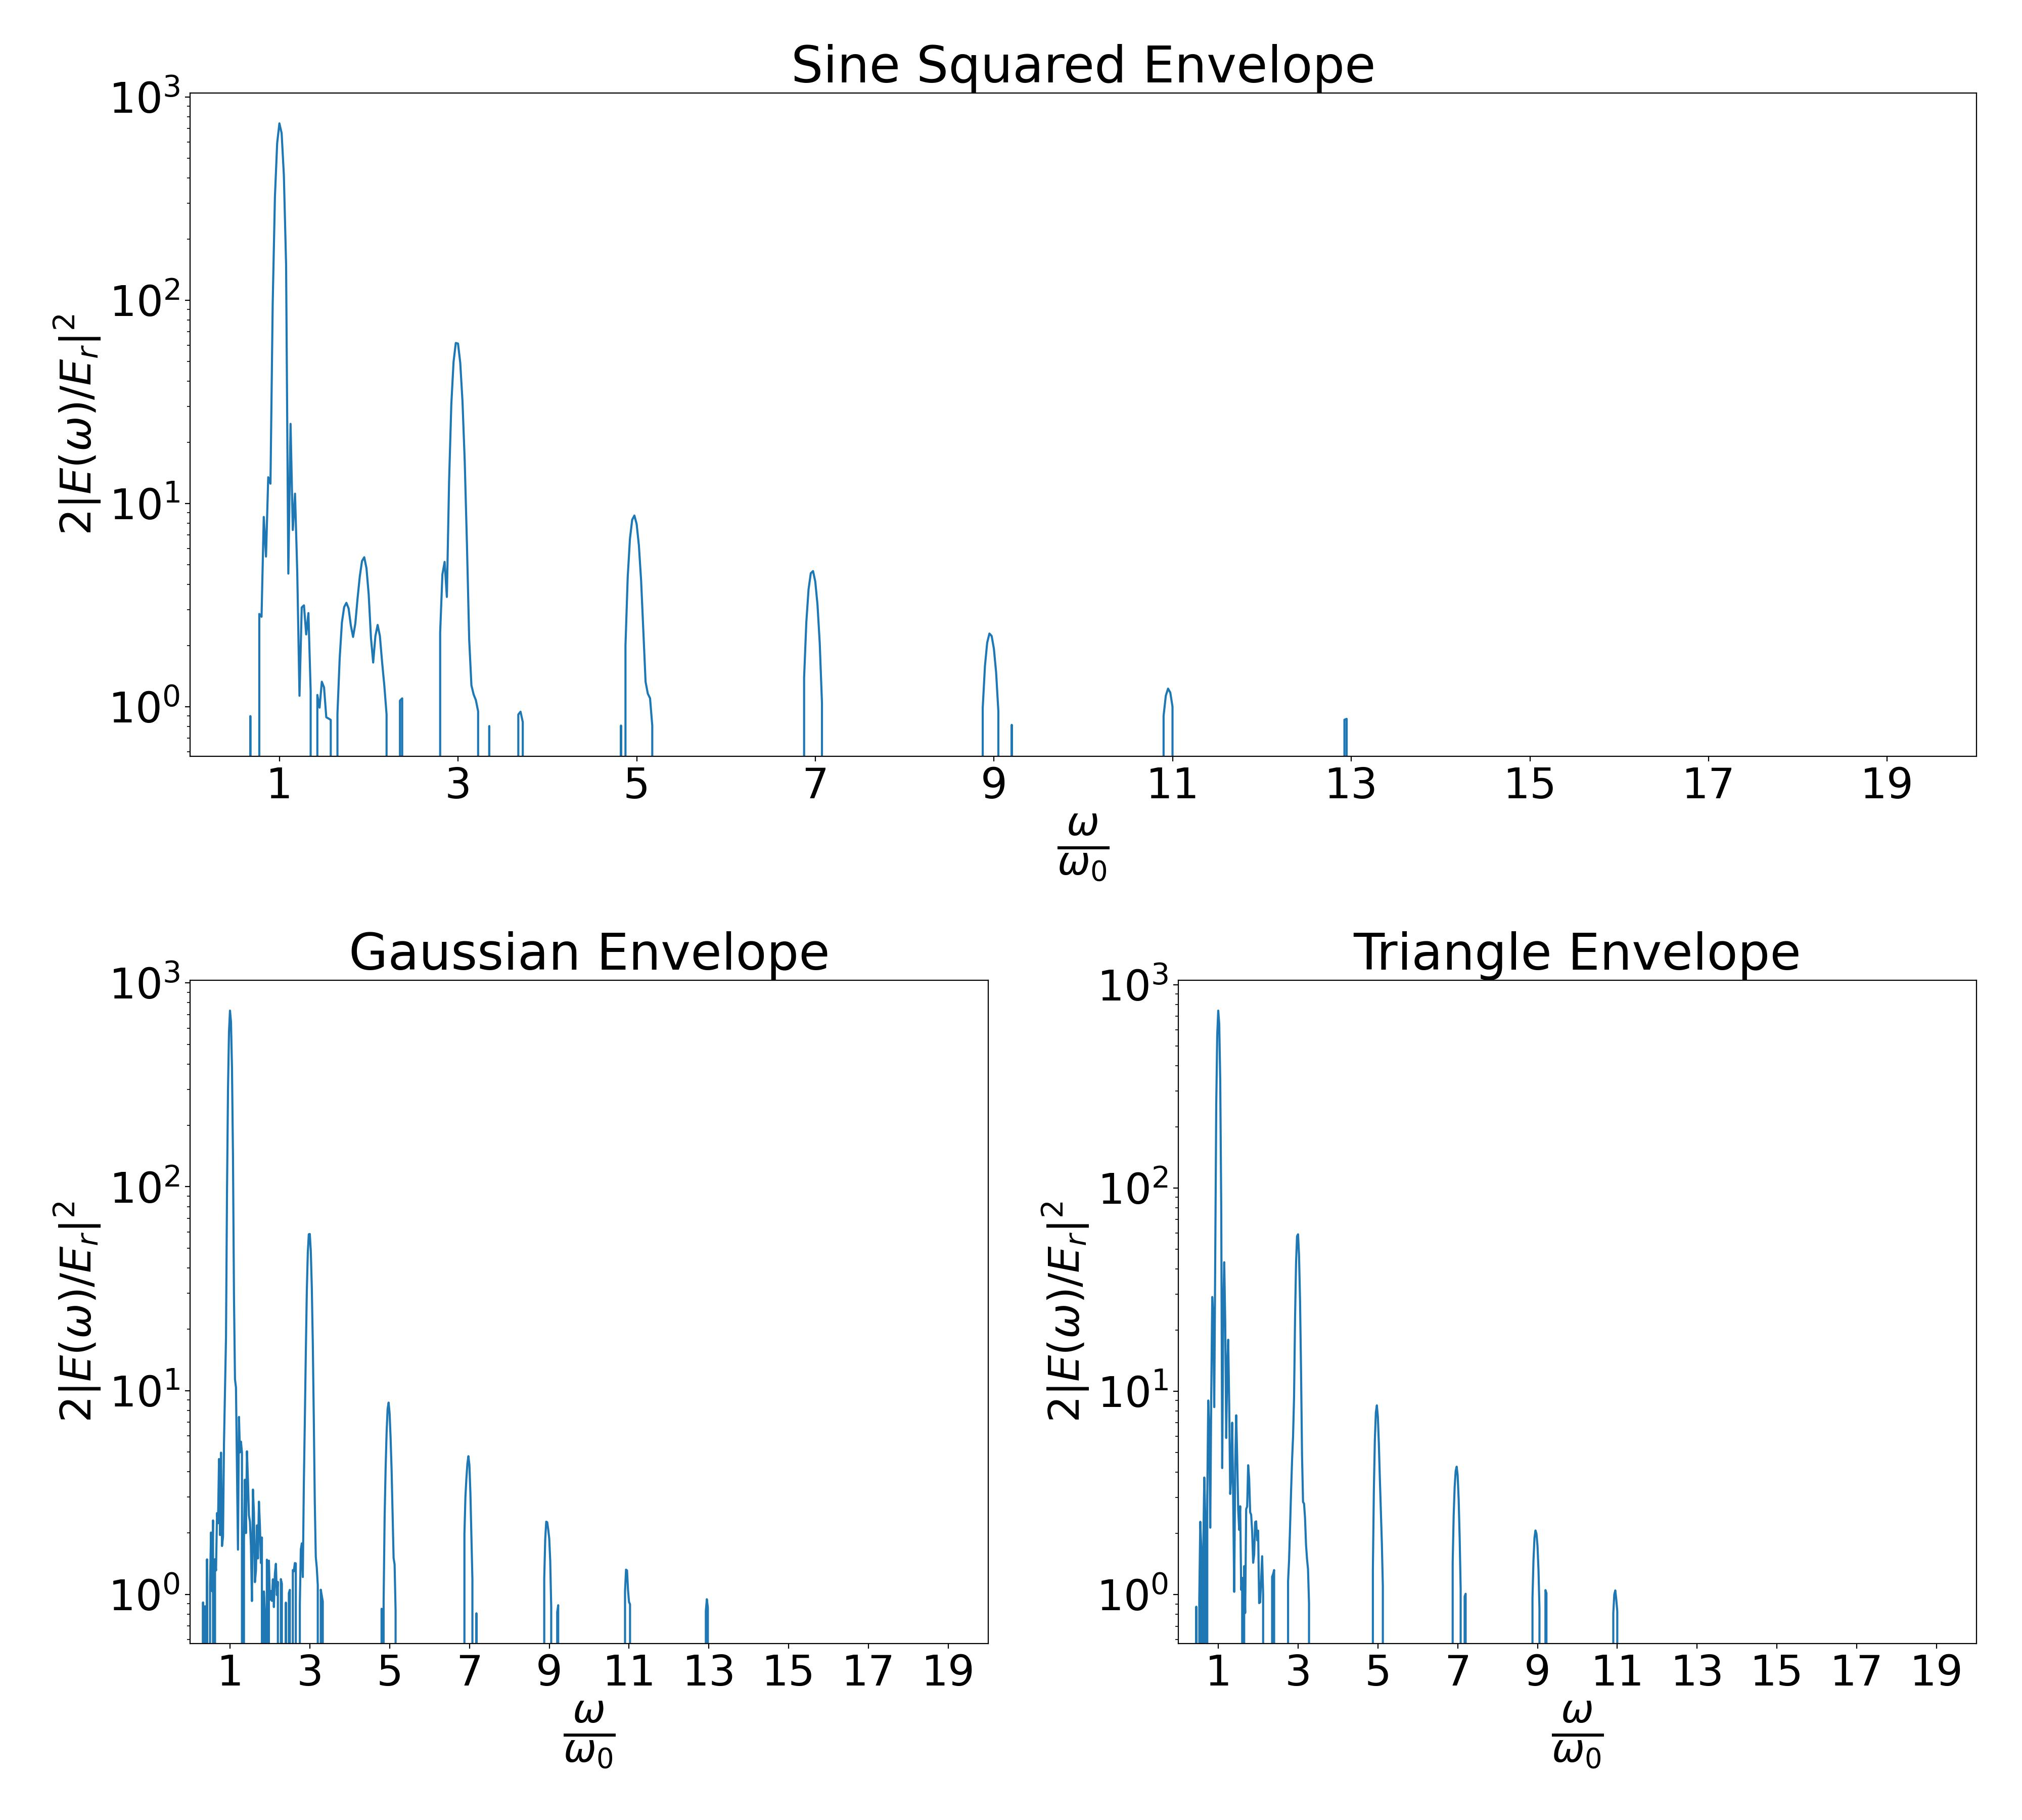
\includegraphics[width=1.0\textwidth, height=0.8\textwidth]{images/env.jpg}
        \caption{Effect of the laser envelope on the harmonics generated.}
        \label{fig:env}
    \end{figure}

    \subsection{Effect of Pulse Duration}
    Increasing the pulse duration increases the number of harmonics generated. The amplitude of the harmonics also increases. The Figure \ref{fig:pulse} on shows the effect of the laser pulse duration on the harmonics generated.
    \begin{figure}[t]
        \centering
        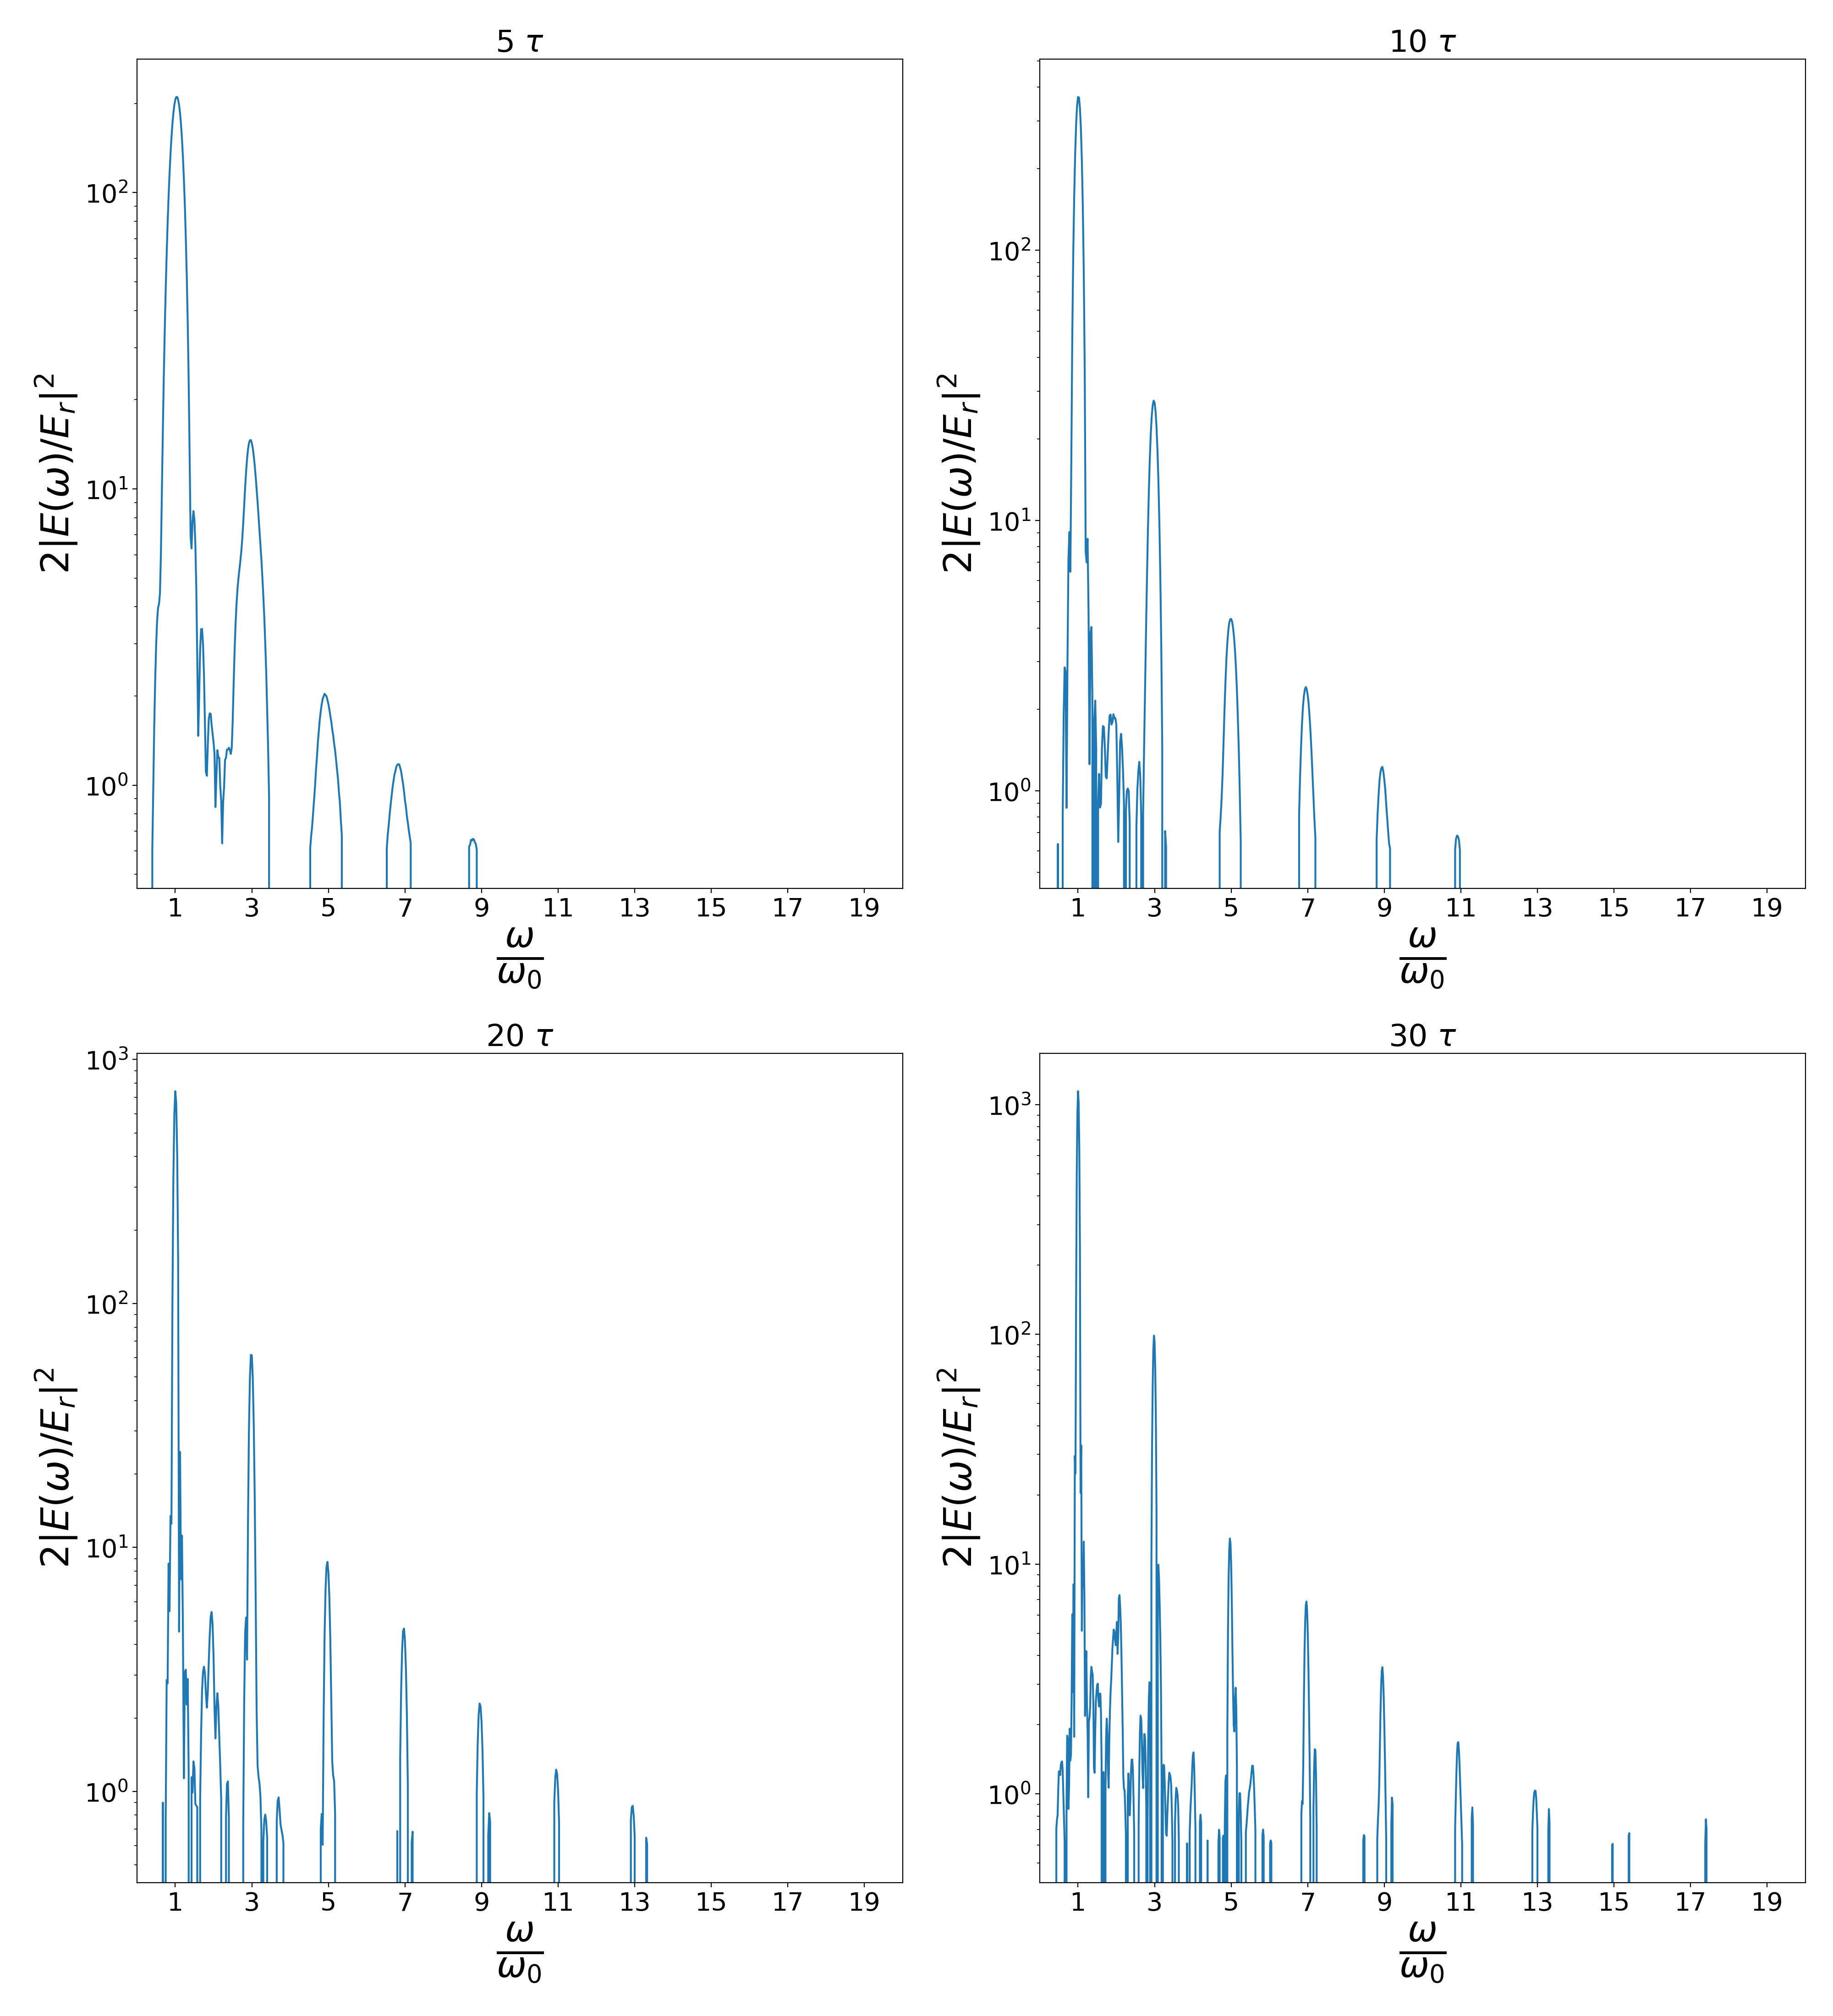
\includegraphics[width=1.0\textwidth, height=0.8\textwidth]{images/pulse.jpg}
        \caption{Effect of the laser pulse duration on the harmonics generated.}
        \label{fig:pulse}
    \end{figure}
    \begin{figure}[t]
        \centering
        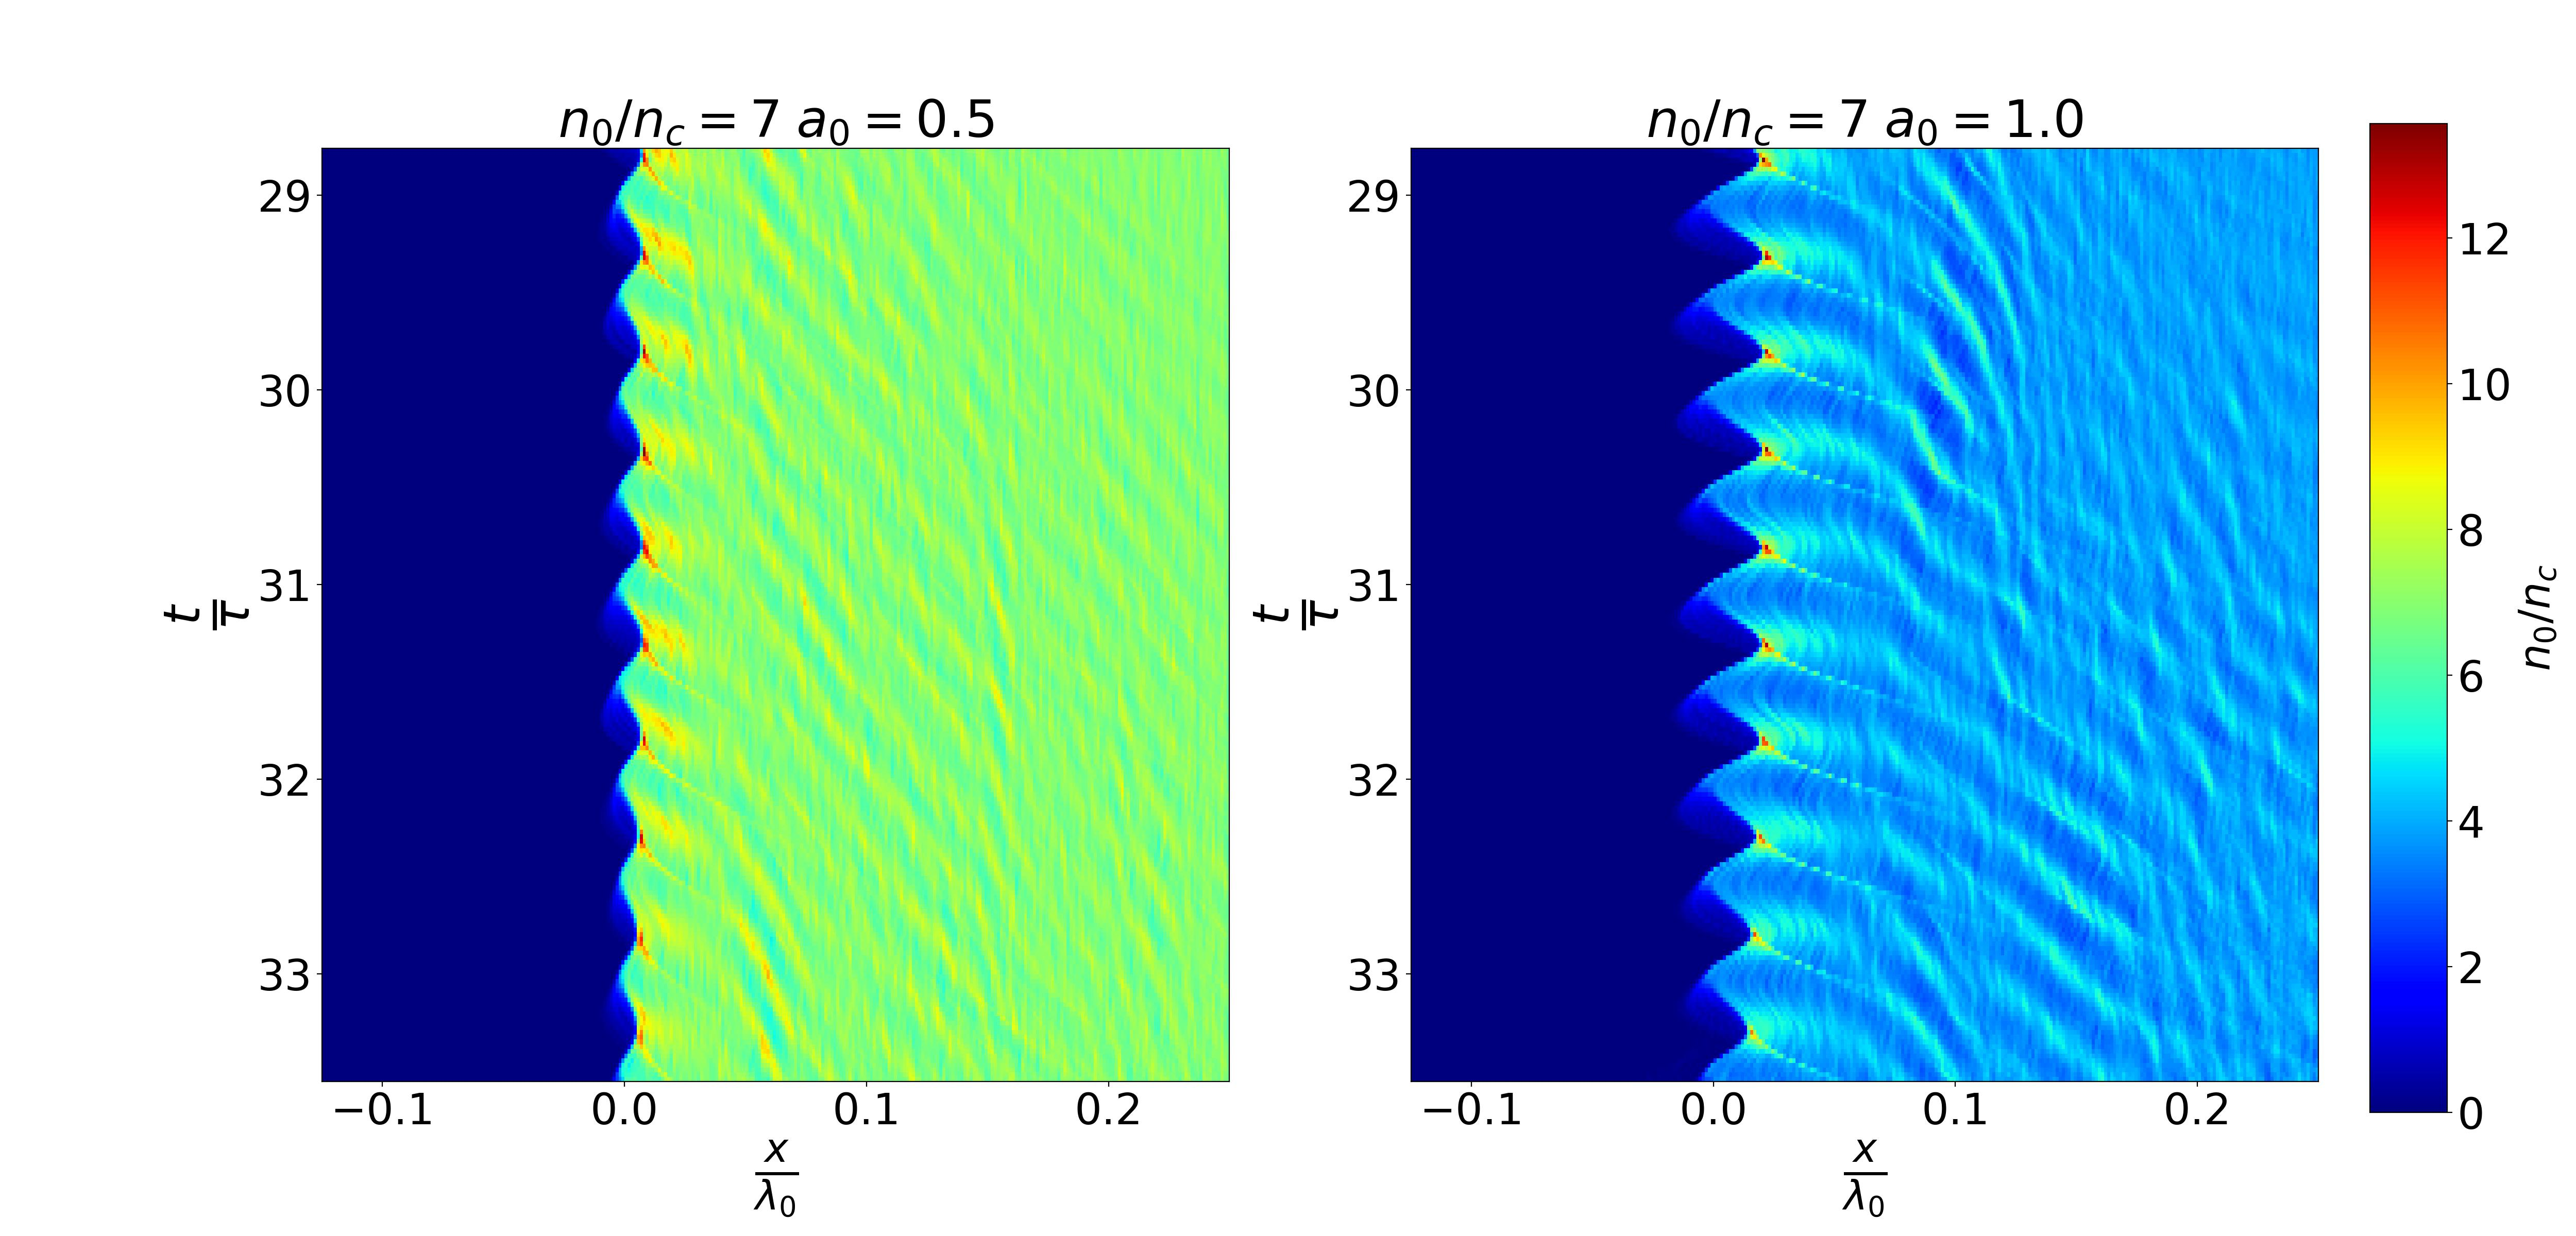
\includegraphics[width=1.0\textwidth, height=0.7\textwidth]{images/oscillation1.jpg}
        \caption{The effect of laser intensity on electron oscillations}
        \label{fig:oscillation1}
    \end{figure}
    \subsection{The Plasma Oscillations}
    In this section, we give some simulation results related to the oscillation of the PM surface.
    \subsubsection{Effect of Laser Intensity on Electron Oscillation}
    The electromagnetic field of high intensity laser beam with plasma makes the electrons inside the plasma oscillate. These oscillations become more and more intetense as the intensity of the EM field increases. (See the Figure \ref{fig:oscillation1})
    \begin{figure}[t]
        \centering
        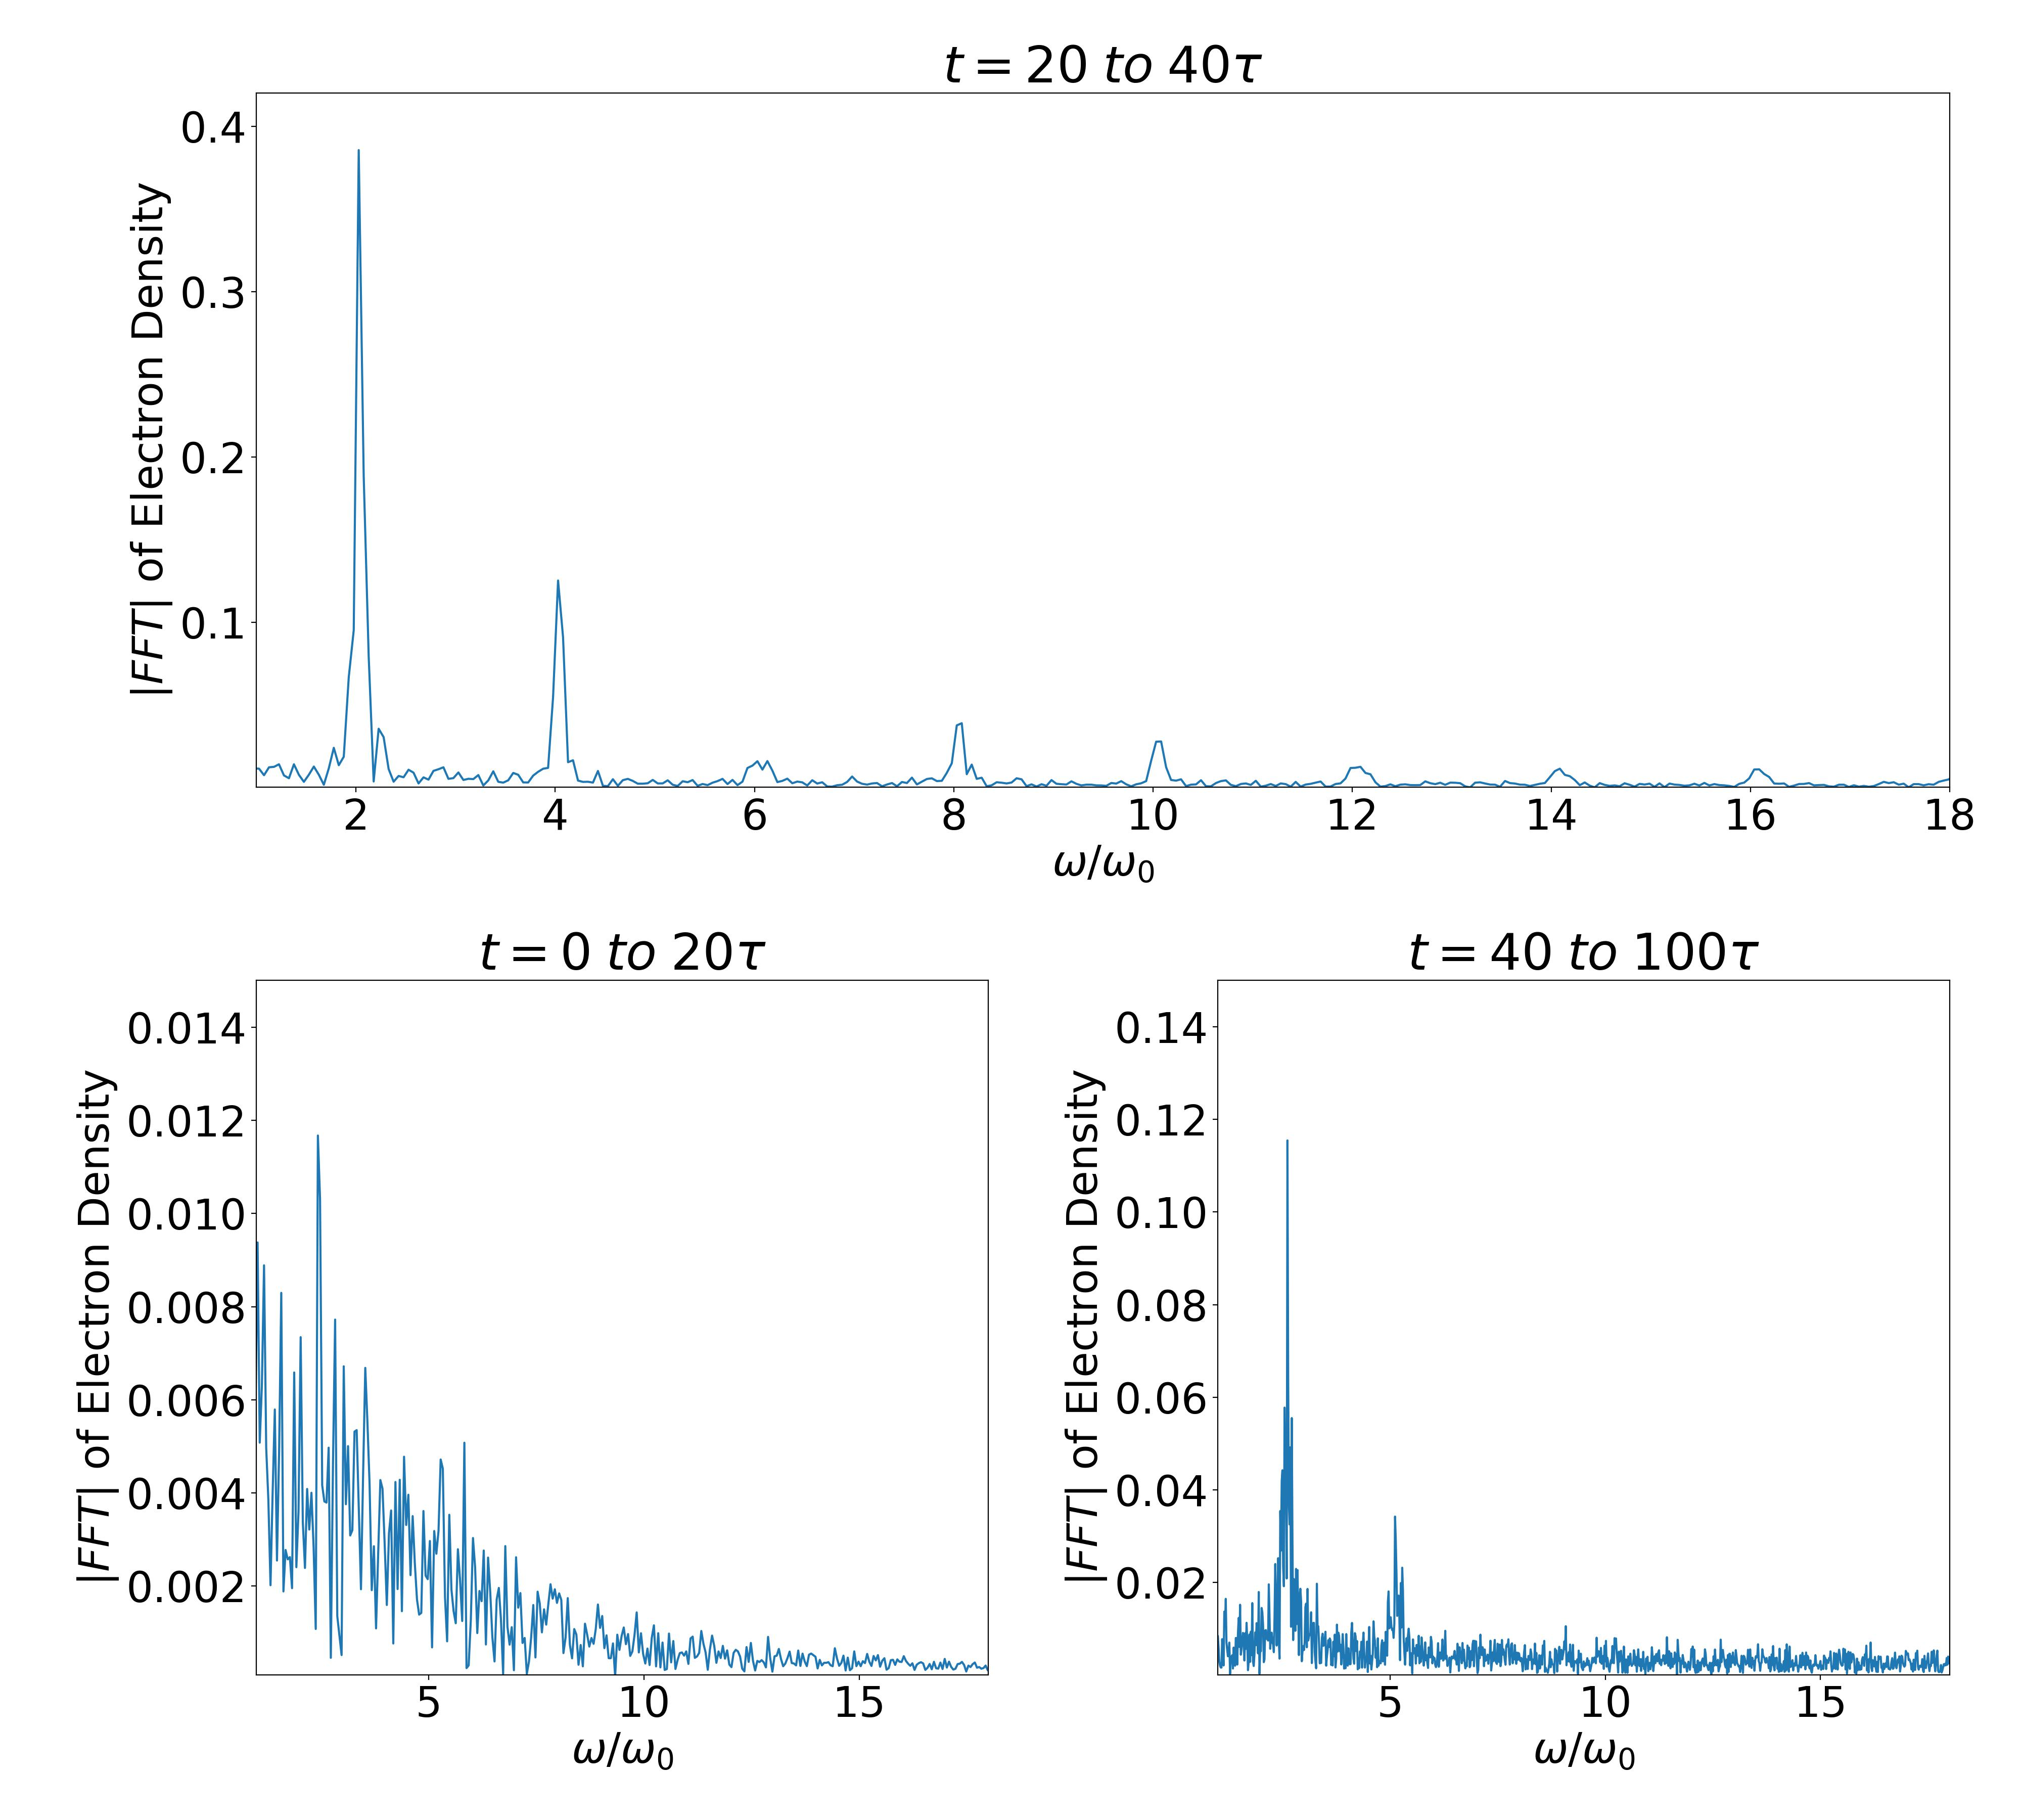
\includegraphics[width=0.9\textwidth, height=0.9\textwidth]{images/oscillation2.jpg}
        \caption{Frequency of electron oscillations during different times}
        \label{fig:oscillation2}
    \end{figure}
    \subsection{The Frequency of Oscillations}
    We found out that the frequency of oscillations is even harmonic of the frequency of the incident laser pulse. Furthermore, electrons are oscillating only till they are interacting with the laser field. (See the Figure \ref{fig:oscillation2})
    \subsection{Theoretical Considerations}
    We use linearly polarized laser pulse and the pondermotive force for this case $\propto \; (1-cos(2\omega_0t))$ which drives the plasma surface twice the laser frequency. We conclude that density is even function.
    Starting from Maxwell's  equation and combining this with equation of motion we get, For normal incidence
    \begin{equation}
        \left (\partial^2 - \frac{1}{c^2}\partial_t^2\right )a = \left (\frac{\omega_p}{c}\right )^2s(x,t)
    \end{equation}
    where $a$ is the vector potential, $s$ is the source term and $\omega_p$ is the plasma frequency. If we assume incident light to be linearly polarized in the z- direction, the source term is given by
    \begin{equation}\label{source}
        s(x,t) = n(x,t)\sqrt{1-\beta_x^2(x,t)}\frac{a_z(x,t)}{\sqrt{1+a_z^2(x,t)}}
    \end{equation}
    Since we are using overdense plasma the major part of the incident light is reflected and the vector potential $a_z(x,t)$  decays rapidly inside the plasma. This can be  approximated by
    \begin{equation}\label{a_z}
        a_z(x,t) \approx \begin{cases}
            -2\mathbf{a_0}\sin(kx-\theta)\sin(\omega t) \; & \text{ for } x < 0   \\
            \mathbf{a_s}\exp(-x/d_s)\sin(\omega t)  \;     & \text{ for } x \ge 0
        \end{cases}
    \end{equation}
    where $d_s = (c/\omega_p)\sqrt{1-(\omega_0 / \omega_p)^2}$\\ \\
    Now, the density $n(x,t)$ is even function. $\sqrt{1-\beta_x^2(x,t)}$ is also an even function while \ref{a_z} is odd function, hence the source function Equation \ref{source} is an odd function. So, normal incidence of lineraly polarized light will generated only odd harmonics. Even harmonic can be found if we use different polarization. \cite{lichters}
    \section{Current Status and Future Plan of Work}
    The interaction of high intensity laser pulse with overdense plasma is investigated. During this, odd harmonics of the incident laser pulse is generated and the effect of variuos laser and plasma parameters on the hormonic generation is studied. Future plan of work is to study about the effects of some more parameters on the harmonics generation escpecially the effect of oblique incidence and different polarization of the laser pulse.
    \section{Acknowledgement}
    % We are very thankful to Prof. Vikrant Saxena for his support and valuable guidance.
    We would want to express our sincere gratitude to our supervisor Prof. Vikrant Saxena for his continous support and for his patience, motivation, enthusiasm and valuable guidance.

    % \bibliographystyle{plain}
    \printbibliography
\end{changemargin}
\end{document}